\documentclass[preprint2,numberedappendix,tighten,twocolappendix]{aastex6}  % USE THIS TO MAKE BIB, THEN FORMAT USING EMULATEAPJ
%\documentclass[twocolumn,apj,numberedappendix]{emulateapj}
\shorttitle{PAPER128 Results}
\shortauthors{Cheng}

\usepackage{amsmath}
\usepackage{graphicx}
\usepackage[figuresright]{rotating}
\usepackage{natbib}
\usepackage{ctable}
\citestyle{aa}

%		Math Shortcuts from Adrian
%\def\b{\mathbf{b}}
%\def\k{\mathbf{k}}
%\def\r{\mathbf{r}}
%\def\q{\mathbf{q}}
%\def\b{\mathbf{b}}
%\def\kp{\mathbf{k}^\prime}
%\def\kpp{\mathbf{k}^{\prime\prime}}
%\def\V{\mathbb{V}}
%\def\At{\tilde{A}}
%\def\Vt{\tilde{V}}
%\def\Tt{\tilde{T}}
%\def\tb{\langle T_b\rangle}
%\newcommand{\vis}{\mathbf{v}}
%\newcommand{\x}{\mathbf{x}}
%\newcommand{\xhat}{\hat{\mathbf{x}}}
%\newcommand{\nhat}{\hat{\mathbf{n}}}
%\newcommand{\A}{\mathbf{A}}
%\newcommand{\N}{\mathbf{N}}
%\newcommand{\rhat}{\hat{\mathbf{r}}}
%\newcommand{\khat}{\hat{\mathbf{k}}}
%\newcommand{\btheta}{\boldsymbol \theta}

\newcommand{\cc}[1]{{\color{purple} \textbf{[#1]}}}

\begin{document}
\title{PAPER128 Results}

\author{
%Aaron R. Parsons\altaffilmark{1,2},
%Adrian Liu\altaffilmark{1,2},
%James E. Aguirre\altaffilmark{3},
%Zaki S. Ali\altaffilmark{1},
Carina Cheng\altaffilmark{1}
%Daniel C. Jacobs\altaffilmark{8},
%David F. Moore\altaffilmark{3},
%Jonathan C. Pober\altaffilmark{1},
}

\altaffiltext{1}{Astronomy Dept., U. California, Berkeley, CA}
%\altaffiltext{2}{Hubble Fellow}
%\altaffiltext{2}{Radio Astronomy Lab., U. California, Berkeley, CA}
%\altaffiltext{3}{Berkeley Center for Cosmological Physics, Berkeley, CA}
%\altaffiltext{3}{Dept. of Physics and Astronomy, U. Pennsylvania, Philadelphia, PA}
%\altaffiltext{8}{School of Earth and Space Exploration, Arizona State U., Tempe, AZ}

\begin{abstract}
\cc{I can write comments like this!}
\end{abstract}


\section{Introduction}
\label{sec:Intro}

%		Notes	
	
%Reference section with: \ref{sec:Intro}
%Reference equation with: \eqref{eq:eqtest}
%Reference figure with: \ref{fig:figtest}
%Cite paper inside sentence: \citet{ref}
%Cite paper at end of sentence: \citep{ref}
%Cite paper inside a parenthetical sentence: \citealt{ref}

%To compile with references shown, compile in BibTeX once and LaTeX twice


%		Sample Equation Syntax
%\begin{equation}
%\label{eqtest}
%\langle \widetilde{T} (\mathbf{k}) \widetilde{T}^* (\mathbf{k^\prime}) \rangle = (2 \pi)^3 \delta^D (\mathbf{k} - \mathbf{k}^\prime) P(k),
%\end{equation}

\section{Observations}
\label{sec:Obs}

\begin{figure}[!]
	\centering
	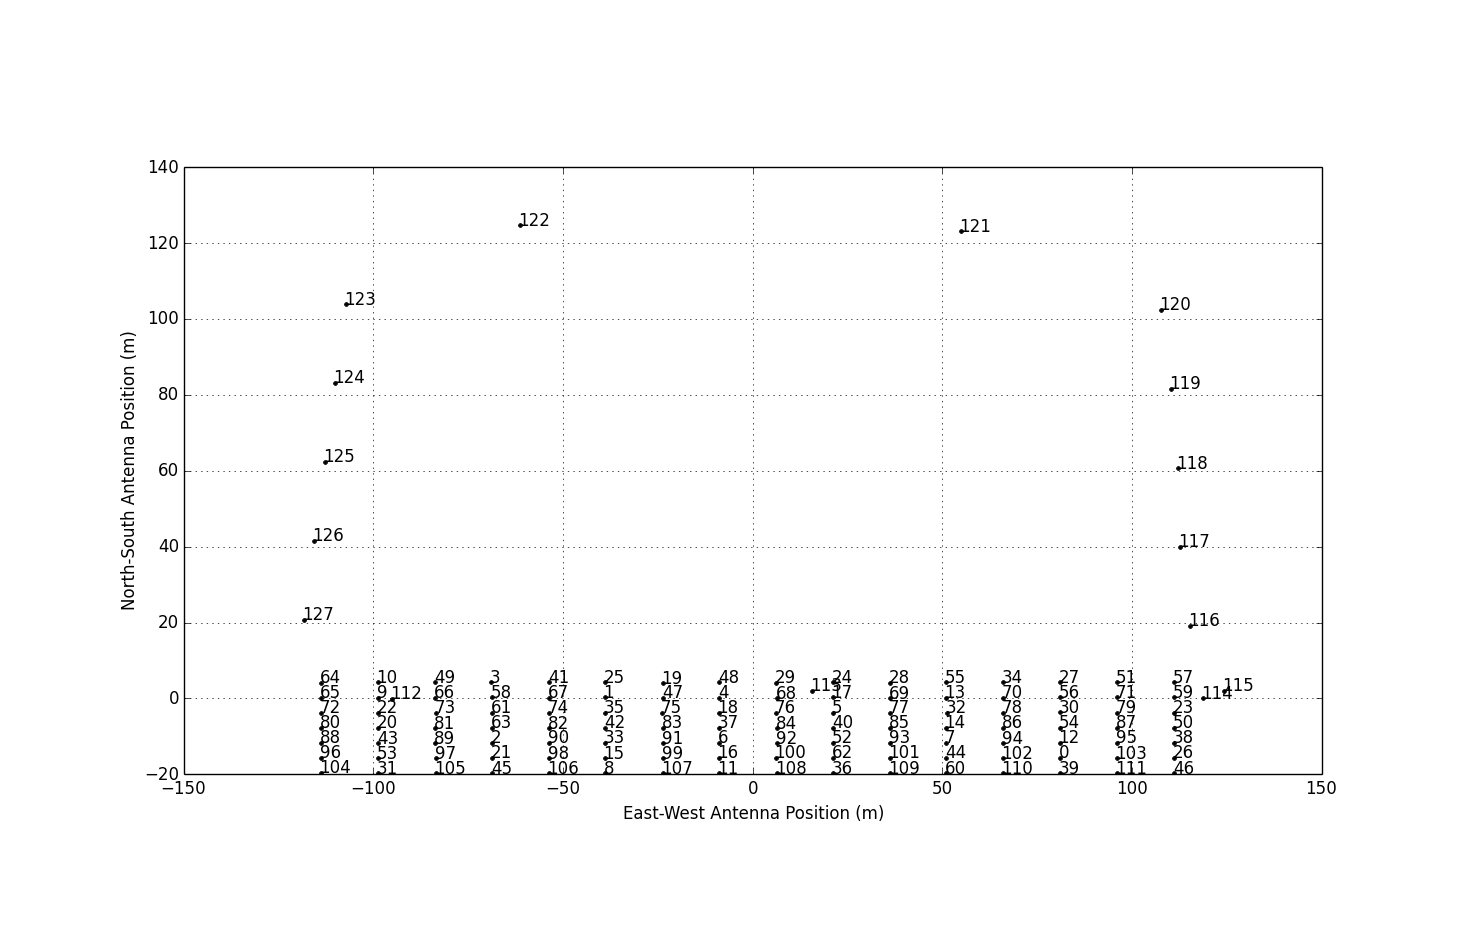
\includegraphics[width=0.52\textwidth]{antlayout.png}
	\caption{\cc{caption here}}
	\label{fig:figtest}
\end{figure}


\section{Data Reduction}
\label{sec:Cal}

\section{Power Spectrum Analysis}
\label{sec:PS}

\subsection{Optimal Quadratic Estimators}
\label{sec:OQE}

\subsection{Signal Loss}
\label{sec:Sigloss}

\section{Results}
\label{sec:Res}

\section{Conclusions}
\label{sec:Con}

\section{Acknowledgements}
\label{sec:Ack}

\bibliographystyle{apj}
\bibliography{refs}


\end{document}

